\documentclass{aims}

%%%%%%%%%%%%%%%%%%%%%%%%%%%%%%%%%%%%%%%%%%
\usepackage{txfonts}
\def\typeofarticle{Type of article}
\def\currentvolume{5}
\def\currentissue{x}
\def\currentyear{2019}
\def\currentmonth{Received date 1 July 2016, Accepted date 6 September}
\def\ppages{xxx--xxx}
\def\DOI{}
\def\Received{xx 2019}
\def\Accepted{xx 2019}
\def\Published{xx 2019}


\newcommand{\ep}{\varepsilon}
\newcommand{\eps}[1]{{#1}_{\varepsilon}}

\numberwithin{equation}{section}
\DeclareMathOperator*{\essinf}{ess\,inf}


\begin{document}
\global\long\def\pardiff#1#2{\frac{\partial#1}{\partial#2}}%

\title{Patient-Specific Estimates of Glioblastoma Multiforme Growth Dynamics
from a Model with Explicit Birth and Death Rates}

\author{%
  Lifeng Han\affil{1},
  Steffen Eikenberry\affil{1},
  Changhan He\affil{1},
  Lauren Johnson\affil{1},
  Mark C. Preul\affil{2},
  Eric J. Kostelich \affil{1},
  and
  Yang Kuang\affil{1,} \corrauth
}

% \shortauthors is used in copyright information in the end of the paper
\shortauthors{the Author(s)}

\address{%
  \addr{\affilnum{1}}{School of Mathematical and Statistical Sciences, Arizona
  State University, Tempe, AZ 85287, USA}
  \addr{\affilnum{2}}{Department of Neurosurgery, Barrow Neurological Institute,
  St.\  Joseph’s Hospital and Medical Center, Phoenix, AZ 85013, USA}}

% corresponding author
\corraddr{kuang@asu.edu}

\begin{abstract}
Glioblastoma multiforme (GBM) is an aggressive primary brain cancer with a
grim prognosis. Its morphology is heterogeneous, but prototypically consists
of an inner, largely necrotic core surrounded by an outer,
contrast-enhancing rim, and often extensive tumor-associated edema beyond.
This structure is usually demonstrated by magnetic resonance imaging (MRI).
To help relate the three highly idealized components of GBMs (i.e.,
necrotic core, enhancing rim, and maximum edema extent) and to the
underlying growth ``laws,'' a mathematical
model of GBM growth with explicit motility, birth, and death processes is
proposed. This model generates a traveling wave solution that mimics tumor
progression.
We develop several novel methods to approximate key characteristics of
the wave profile, which can be compared with MRI data. Several simplified
forms of growth and death terms and their parameter identifiability are
studied.  We use several test cases of MRI data of GBM patients to
yield personalized parameterizations
of the model, and the biological and clinical implications are discussed.
\end{abstract}

\keywords{Glioblastoma multiforme; parameter estimation;
reaction-diffusion models; patient-specific models.}

\maketitle

\section{Introduction}

Glioblastoma multiforme (GBM) is a highly aggressive primary brain cancer,
with median survival time from diagnosis on the order of 15 months;
long-term survival is extremely rare \cite{Norden2006}.  Such rapid
progression is promoted by highly proliferative and diffusely invasive
cancer cells, which makes complete surgical removal impossible. Magnetic
resonance imaging (MRI) is conventionally used to identify the location and
characteristics of the tumor pre-operatively, to guide surgery, and to
monitor and track progression and treatment response. Perioperatively, MRI
is used to guide the resection of the tumor mass, to assess post-operatively
the volume of tumor resected, and to target other adjunct treatment such as
radiation therapy.

GBMs morphologically typically appear (at least at initial diagnosis) as
roughly spherical but highly heterogeneous masses that often exhibit a
(crudely speaking) three-layer structure.  Within the tumor there is usually
extensive cell necrosis, often accompanied by tumor cells, and a cystic
component as well.  An outer region, which typically appears as
contrast-enhancing on T1-weighted gadolinium contrast-enhanced MRI, is
cytologically typified by proliferating cells that then infiltrate into
surrounding brain tissue.  The surrounding brain tissue is generally seen to
be edematous on T2-weighted or T2-FLAIR MRI and at surgery, due to vasogenic
edema.  Prior statistical analyses have found that edema is a prognostic
indicator of patient survival~\cite{Pope2005}, but the relationship is
complex and appears to be mediated by the expression of vascular endothelial
growth factor and the activity of related angiogenic
genes~\cite{Carlson2007} and various autocrine
factors~\cite{Hoelzinger2007}.

The standard of care for GBM patients was largely established by the 2005
clinical trial by Stupp \emph{et al.}~\cite{Stupp2005}.  It comprises
maximal surgical resection of the primary tumor, followed by six weeks of
radiation to the gross tumor volume, plus a 2--3~cm margin, with concomitant
oral temozolamide (TMZ), and 6--12 months of maintenance TMZ chemotherapy~\cite{Gilbert2013}.  Maximal surgical resection
appears to offer some
survival benefit.  Nevertheless, the absolute survival benefit of even the
most effective therapy is typically on the order of months.  The highly
infiltrative nature of GBMs makes recurrence nearly inevitable,
even with maximal resection and aggressive adjuvant therapy,
although individual tumors vary in their degree of invasiveness.

Given the grim situation, mathematical modeling has been proposed as a
method to better understand the biophysical rules underlying GBM growth,
with the ultimate goal to provide more effective therapy.  Mathematical
models have been widely applied to a variety of cancers and to cancer
treatment in general~\cite{Kuang}, and GBM is the focus of many such works
(see \cite{Martirosyan2015} for a review).  A popular class of cancer models
takes the form of a system of reaction-diffusion equations. In many cases
\cite{Harley2014,Gerlee2016,Stepien2018}, such systems generate a traveling
wave solution, with the traveling wave speed of great interest, as it is an
indicator of how fast the cancer progresses.

Variants of the Fisher-Kolmogorov equation~\cite{Fisher1937}, originally introduced
in the 1930s, were first suggested (to our knowledge)
as models for GBM growth by J.~D. Murray and coworkers.
The Fisher-Kolmogorov model is given by
\begin{equation}
\pardiff{c}{t} = \nabla\cdot\left(D \nabla{c}\right) + \rho c \left(1 - \frac{c}{K}\right),
\label{fisher-eq}
\end{equation}
where $c(x,t)$ is the cancer cell density at location $x$ and time $t$, $D$
is a diffusion coefficient, $\rho$ is the intrinsic tumor cell growth rate,
and $K$ is the local carrying capacity.  (Variants include a linear version
that replaces the logistic growth term with a simple exponential growth
rate, $\rho c$.)  Murray and coworkers have used them to explore the effect of
chemotherapy~\cite{Tracqui1995}, to quantify patients' survival as a function
of the extent of surgical resection~\cite{Woodward1996},
and to estimate the time of tumor initiation~\cite{Murray2012}.

Other authors have suggested that the net growth and diffusion parameters
of model~(\ref{fisher-eq}) may be estimated by image differencing when
two sequential, pre-treatment patient MR series are
available~\cite{Swanson2008,Neal2013,Jackson2015a}.
Such a procedure is problematic, however, because changes in
the tumor in images taken a few days or weeks apart tend to be small
and are convolved with image co-registration errors~\cite{vanderHorn2016}.
Some patients may be treated with
steroids following initial diagnosis to reduce tumor-related edema and
resulting neurological symptoms,
which may alter the brain geometry and imaging appearance of the
tumor at subsequent times~\cite{Watling1994,Zaki2004}.

Model~(\ref{fisher-eq}) can yield a dense tumor
core with an advancing front, but it cannot capture the heterogeneity between
live and necrotic tumor cells, as it assumes that all cells are equally
viable.  While several modeling efforts have taken into account various
proliferating, migrating, and necrotic cell components (e.g.,
\cite{Eikenberry2009,Swanson2011}), they are too complicated to be reliably
parameterized by the limited number of patient MRI series in typical
clinical cases.  The motivation for this work is to extend model~(\ref{fisher-eq})
to include necrotic cells in a simplified way, such that
patient-specific model parameters can be estimated from suitable measurements of MR
images acquired at a single time point.

T1-weighted MRI sequences of GBM often show a partially necrotic core
surrounded by a bright enhancing rim that correlates with high blood vessel
density and, presumably, with rapid cell proliferation. Neurosurgical and biopsy
studies indicate that this core and
rim are usually surrounded by a large expanse of edema, which is best visualized
on T2-weighted MRI and has been found to correspond with a component of diffusely
invasive GBM cells~\cite{Claes2007}.  By approximating the tumor as a sphere, we
may be able to identify three \emph{idealized} digital marks from imaging:
necrotic radius, enhancing radius, and what we shall call the ``T2'' or
``maximum'' radius.  We hypothesize that a relatively simple mathematical model
framework can capture all these three digital marks and yield insights into the
relative contributions of cellular proliferation, motility, and necrosis to the
observed image features.

The next section describes our model and its
assumptions.  We demonstrate that the model has a traveling wave solution
and present the approximate wave profile.  We describe a simple procedure to
estimate patient-specific parameters by fitting the approximate wave profile to a
tumor profile derived from patient MRIs. The identifiability of the model
parameters is also discussed. We apply this parameter estimation procedure to
obtain the key model parameters (consisting of the rate of cancer
cell proliferation, death, and diffusion) for several patients.


\section{Model and method}

\subsection{Model description}
\label{model-sec}
Our proposed model of the growth of GBM is a system of reaction-diffusion
equations:
\begin{subequations}\label{eq:main3d}
\begin{eqnarray}
\pardiff{p}{t} & = & \nabla\cdot\left[\left(\frac{Dp}{p+q}\right)
  \nabla(p+q)\right]+\tilde{g}(w)p-\tilde{\delta}(w)p,\label{eq:main3d1}
  \\[\medskipamount]
\pardiff{q}{t} & = & \nabla\cdot\left[\left(\frac{Dq}{p+q}\right)
  \nabla(p+q)\right]+\tilde{\delta}(w)p, \label{eq:main3d2}
\end{eqnarray}
\end{subequations}
where
\begin{equation}
w = 1 - p - q,
\label{w-eq}
\end{equation}
and $p(x,t)$ and $q(x,t)$ represent the proliferating and quiescent cell
densities at time $t$ and location~$x$, respectively; quiescent cells are
functionally equivalent to necrotic cells in this framework.
We assume that the flux of total population due to migration is $-D\nabla(p+q)$,
where $D$ is a constant diffusion coefficient. It is further assumed
that the proportion of the total flux contributed by each cell type
equals its proportion of the total population. This form of diffusion was used in
\cite{Sherratt2001b} to account for the key property of contact inhibition in
cancer cell movement, with the underlying assumption that the two cell
populations move together with equal motility, unaffected by necrotic cells. This
type of model has successfully captured the structure of a growing tumor.

The per capita birth rate is $\tilde{g}(w)$; proliferating cells
become quiescent at the per capita rate $\tilde{\delta}(w)$, where $w$
(Eq.~\ref{w-eq})) represents the availability
of space or some generic nutrient, which we call ``growth factor'' henceforth.
We have scaled the maximum cell density to be~$1$. In our
model, necrosis is not explicitly included but can be regarded as being
lumped into~$q$.  Insofar as quiescent cells cannot become proliferative,
$\tilde{\delta}(w)$ can be viewed as a functional death rate.  Our motivation in
keeping the model framework relatively simple is to be
able to estimate model parameters directly from clinical MRI imaging that is
sparse in time.

To make the model biologically reasonable, we impose the following constraints on $g(w)$ and $\delta(w)$:
\begin{equation}
\tilde{g}'(w)\ge0,\quad
\tilde{\delta}'(w)\le0,\quad
\tilde{g}(1)\ge\tilde{\delta}(1)=0,\quad
\tilde{\delta}(0)>\tilde{g}(0)=0.
\label{eq:1assume}
\end{equation}
That is, birth (death) should increase (decrease) with the availability of
the growth factor, there is more birth than death at maximum values of
the growth factor, and there is only death with no growth in the 
absence of growth factor. 
It is also assumed that the death rate is negligible at maximum values of
the growth factor.  With these assumptions, we observe numerically that with suitable initial conditions, the solution of (\ref{eq:main3d}) stays positive and is bounded ($p+q\le 1$) for all~$t$. 

We can estimate only up to three parameters based on the necrotic,
enhancing, and maximum radii to be measured
from MRI images.  Therefore, we place a few more
restrictions on $\tilde{g}(w)$ and $\tilde{\delta}(w)$ to simplify
the estimation of model parameters and to ensure their identifiability.
We assume that the proliferation rate at maximum growth factor is $\rho$
and that the death rate at zero growth factor
is~$k$ and incorporate these parameters into $\tilde{g}$ and
$\tilde{\delta}$, respectively; that is,
$\tilde{g}(w=1;\rho)=\rho$ and $\tilde{\delta}(w=0;k)=k$.
For reasons that will become clear later, we pick a functional form
that can be written as $\tilde{g}(w;\rho)=\rho g(w)$ and 
$\tilde{\delta}(w;k)=k\delta(w)$.
Some examples include the cumulative distribution function of the beta 
distribution family (cf.\ the left pane of Figure~\ref{fig:beta26f}).
These additional assumptions impose little impact on the generality 
of our model. The benefit of including them will become
clear in Section~\ref{paramest-sec}.

\subsection{Approximate wave profile}

In most biological applications of reaction-diffusion models, solutions 
take the form of traveling waves. MRI images of GBM cancer growth suggest
that we can approximate the evolution of the tumor by a traveling-wave
solution of its growth model.
To uniquely identify and accurately approximate GBM growth model parameters,
it is highly desirable to obtain some analytic approximation of the
traveling wave, to enable computational matching of the image wave profile
and the approximate model wave profile.
For this purpose, we consider one spatial dimension, which suffices
insofar as the tumor is approximately spherical, and, at the time of
diagnosis, its radius is large enough so that radial effects are negligible.
With these assumptions, model~(\ref{eq:main3d}) takes the form
\begin{subequations}\label{eq:main}
\begin{eqnarray}
\pardiff{p}{t} & = &
  \pardiff{}x\left[\left(\frac{Dp}{p+q}\right)\pardiff{}x(p+q)\right]+
  \rho g(w)p-k\delta(w)p \\[\medskipamount]
\pardiff{q}{t} & = &
  \pardiff{}x\left[\left(\frac{Dq}{p+q}\right)\pardiff{}x(p+q)\right]+
  k\delta(w)p.
\end{eqnarray}
\end{subequations}
We nondimensionlize the system using the characteristic
length $\sqrt{D/k}$ and the characteristic time $1/k$ so that
$x=\sqrt{D/k}\,\hat{x}$ and $t=\hat{t}/k$, which leads to
\begin{subequations}\label{eq:main1d}
\begin{eqnarray}
\pardiff{p}{\hat{t}} & = &
  \pardiff{}{\hat{x}}\left[\left(\frac{p}{p+q}\right)
    \pardiff{}{\hat{x}}(p+q)\right]+\hat{\rho}g(w)p-\delta(w)p \\[\medskipamount]
\pardiff{q}{\hat{t}} & = &
  \pardiff{}{\hat{x}}\left[\left(\frac{q}{p+q}\right)
    \pardiff{}{\hat{x}}(p+q)\right]+\delta(w)p,
\end{eqnarray}
\end{subequations}
where $\hat{\rho}=\rho/k$. We seek a traveling
wave solution of the form $p(\xi)=p(\hat{x}-c\hat{t})$,
$q(\xi)=q(\hat{x}-c\hat{t})$, where $c$ is the wave speed.
Substituting these into (\ref{eq:main1d}) gives
\begin{subequations}\label{eq:wavecoord}
\begin{eqnarray}
\frac{d}{d\xi}\left[\left(\frac{p}{p+q}\right)\frac{d}{d\xi}(p+q)\right]+
  c\,\frac{dp}{d\xi}+ \hat{\rho}g(w)\,p-\delta(w)\,p & = & 0 \\[\medskipamount]
\frac{d}{d\xi} \left[\left(\frac{q}{p+q}\right)\frac{d}{d\xi}(p+q)\right]+
  c\,\frac{dq}{d\xi}+\delta(w)\,p & = & 0.
\end{eqnarray}
\end{subequations}
Linearizing at the wave head, i.e., substituting the
ansatz $p=Ae^{-r\xi}$ and $q=Be^{-r\xi}$ into (\ref{eq:wavecoord}),
gives $(r^{2}-cr+\rho)A=0$.
For a biologically realistic wave front, we expect $A>0$, $B>0$, and $r>0$.
This requires that $c^2>4\rho$, which implies that the minimum
speed of the wave is $c_{\mbox{\scriptsize min}}=2\sqrt{\hat{\rho}}$. 
It is numerically verified that the minimum speed is exactly the
asymptotic speed, i.e., $c=c_{\mbox{\scriptsize min}}$.


To obtain an approximate wave profile, we adopt a method first used
by Canosa~\cite{Canosa1973}. We rescale the wave coordinate as $z=-\xi/c$,
which leads to
\begin{subequations}\label{eq:1/c^2}
\begin{eqnarray}
\frac{1}{c^{2}}\,\frac{d}{dz}\left[
  \left(\frac{p}{p+q}\right)\frac{d}{dz}(p+q)\right]
   -\frac{dp}{dz}+\hat{\rho}g(w)\,p-\delta(w)\,p & = & 0,
   \label{eq:1/c^2a} \\[\medskipamount]
\frac{1}{c^{2}}\,\frac{d}{dz}\left[\left(\frac{q}{p+q}\right)
   \frac{d}{dz}(p+q)\right]- \frac{dq}{dz} +\delta(w)\, p & = & 0. \label{eq:1/c^2b}
\end{eqnarray}
\end{subequations}
Assuming that $1/c^{2}$ is small, we neglect each first term
of (\ref{eq:1/c^2}). Writing the resulting system in terms
of $p$ and~$w$, we obtain the reduced system
\begin{subequations}\label{eq:pp system}
\begin{align}
\frac{dp}{dz} & =p\,\bigl(\hat{\rho}g(w)-\delta(w)\bigr),
   \label{eq:dpdz} \\[\medskipamount]
\frac{dw}{dz} & =-\hat{\rho}\,pg(w),\label{eq:dwdz}
\end{align}
\end{subequations}
which is amenable to phase plane analysis. The
approximate wave solution corresponds to a trajectory that leaves
$(0,1)$ and ends at $(0,w^{*})$, with $w^{*}\in[0,1)$ 
(see Figure~\ref{fig:pp}).  (In the appendix, we show that such a trajectory
exists, given the assumptions~(\ref{eq:1assume}).)
Dividing (\ref{eq:dpdz}) by (\ref{eq:dwdz}) yields
\begin{equation} 
\label{eq:dpdw}
\frac{dp}{dw}=\frac{\delta(w)}{\hat{\rho}\,g(w)}-1.
\end{equation}
Upon integration, we obtain $p$ as a function of~$w$, which we will
use in the next section.

\begin{figure}
\begin{center}
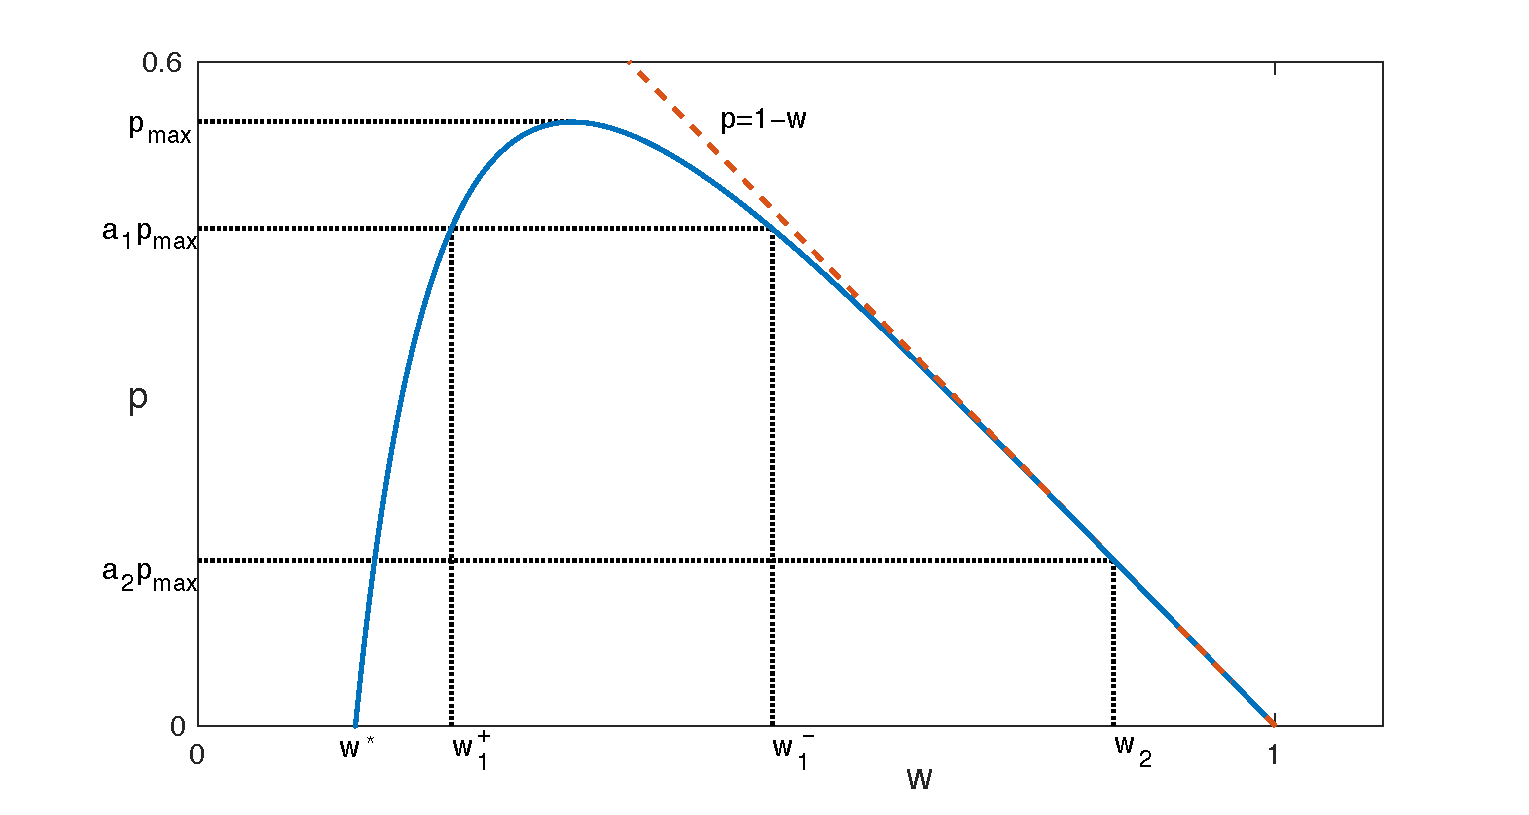
\includegraphics[scale=0.55]{plots/pp-edited.pdf}
\end{center}
\caption{A typical trajectory that connects $(0,1)$ and $(0,w^*)$ in the phase plane. Given $\delta(w)$ and $g(w)$, this trajectory can be found by integrating~(\ref{eq:dpdw}).  It represents an approximate traveling wave solution.  See the appendix for a proof of its existence under general assumptions.}
\label{fig:pp}
\end{figure}


\subsection{Parameter estimation}
\label{paramest-sec}

From clinical MRI data, we may derive three idealized radii:
$R_{0}$, $R_{1}$, and $R_{2}$, representing respectively the radius of the
inner necrotic core, the radius to the edge of the contrast-enhancing rim,
and the radius to the outer edge of tumor-associated edema.  Such data have
been extracted from a series of anonymized patient MRI data consisting of
T1-contrast enhanced and T2-weighted MRIs at initial diagnosis.  Using
SPM~12 \cite{Penny2007}, MRIs are initially registered to a standard brain
space, and then, using Slicer~3D \cite{Fedorov2012}, the total necrotic core
volumes, enhancing rim volumes, and tumor-associated edema volumes are
determined from semi-manual tumor segmentation.  Finally, these volumes are
converted to radii assuming a spherical tumor geometry.  The width of the
proliferating rim, denoted as~$L_{1}$, and the width of the edematous rim,
denoted as~$L_{2}$, can be calculated as $L_{1}=R_{1}-R_{0}$ and
$L_{2}=R_{2}-R_{1}$, as demonstrated visually in
Figures~\ref{fig:radii_process} and~\ref{fig:matchwidth}.

We assume that contrast-enhancing regions of T1-weighted images
correspond to high densities of proliferating tumor cells and that edematous
regions on T2-weighted imaging correspond to low densities.  We denote the
respective detection thresholds for T1 and T2 imaging as
$a_1p_{\mbox{\scriptsize max}}$ and $a_2 p_{\mbox{\scriptsize max}}$,
where $0 < a_2 < a_1 < 1$ and 
$p_{\mbox{\scriptsize max}}=\max_{z} p(z)$,
i.e., the maximum density of proliferating cells given by the traveling wave
solution.

Often only a single MRI series is available before surgery, although in some
cases, a diagnostic MRI followed some days or weeks later by a pre-surgery MRI
may be available.  In the latter case, the
image-derived wave velocity $V$ is the change in tumor radius divided
by the length of the time interval.

From our approximate wave profile, we can compute the corresponding
quantities to match with MR images (cf.\ Figure~\ref{fig:matchwidth}). The
rim width (in dimensional form) is computed as
\begin{subequations}
\begin{eqnarray}
\ell_{1} & = & \frac{2\sqrt{D\rho}}{k}
  \int_{w_{1}^{-}}^{w_{1}^+} \frac{dz}{dw} \,dw,\label{eq:l1}\\
\ell_{2} & = & \frac{2\sqrt{D\rho}}{k}
  \int_{w_{2}}^{w_{1}^-} \frac{dz}{dw}\, dw,\label{eq:l2}
\end{eqnarray}
\end{subequations}
where $w_{1}^{\pm}$ and $w_{2}$ satisfy, respectively,
$p(w_{1}^{\pm})=a_{1}p_{\mbox{\scriptsize max}}$ and
$p(w_{2})=a_{2}p_{\mbox{\scriptsize max}}$.  Here
$p(w)$ is obtained by integrating Eq.~(\ref{eq:dpdw}) (see appendix for details).
Additionally, the model-derived wave speed $c=2\sqrt{\rho D}$
can be matched with image-derived speed
$V$. Thus we have three nonlinear equations
\begin{equation}
\ell_{1}=L_{1},\quad \ell_{2}=L_{2},\quad c=V,
\label{eq:l1l2c}
\end{equation}
from which we hope to find the parameters $D$, $\rho$, and~$k$.  Given our
assumptions, we can simply take the ratio of
(\ref{eq:l1}) and (\ref{eq:l2}), which gives
\begin{equation}
f(\hat{\rho})\equiv
\frac{\displaystyle\int_{w_{1}^{-}}^{w_{1}^{+}}\frac{dz}{dw}\,dw}
  {\displaystyle\int_{w_{2}}^{w_{1}^{-}}\frac{dz}{dw}\,dw}=
  \frac{L_{1}}{L_{2}},
\label{eq:frhohat}
\end{equation}
insofar as the integrals are functions of~$\hat{\rho}$. 
Equation~(\ref{eq:frhohat})
can be solved for $\hat{\rho}$ analytically in special cases or numerically
in general.  The monotonicity of $f(\cdot)$ is important
for the identifiability of parameters. Once we find~$\hat{\rho}$, i.e., the ratio 
$\rho/k$, all parameters can be found by back substitution.

The above method requires two MR scans taken at two consecutive times
prior to surgery to obtain an image-derived estimate of wave speed. If no
second MR series is available, then tumor age may be estimated by the
tumor radius divided by the wave speed. However, the estimate depends on
which radius ($R_{1}$ or $R_{2}$) is used, because the tumor grows
exponentially at first and linearly later on~\cite{Kuang}. This
initial exponential growth stage needs to be taken into account as
a correction to the aforementioned tumor age estimation.  Suppose that for
$0\le t\le t^*$, quiescence is negligible and the proliferating cancer cells grow
exponentially from a point source of density~$p_0$, and that for  $t > t^*$,
the tumor grows as a traveling wave with speed $2\sqrt{\rho D}$. 
By equating the two age estimates, we obtain
\begin{equation}
\label{eq:age est}
\frac{R_1-R_1^*}{2\sqrt{\rho D}} =  \frac{R_{2}-R_2^*}{2\sqrt{\rho D}},
\end{equation} 
where 
\begin{equation} \label{eq:Rstar}
R^*_{i} = t^* \sqrt{4D\rho - \frac{4D}{t^*} \ln\left(
  \frac{a_i ( 4\pi D t^*)^{3/2}}{p_0} \right)},\qquad i=1,2,
\end{equation}  
where $R_1$ and $R_2$ are respectively the T1 and T2 radii at $t=t^*$ 
(see details of $R_1^*$ and $R_2^*$ in the appendix). 

Replacing the last equation in (\ref{eq:l1l2c})
with (\ref{eq:age est}), we again have three equations. To solve them
for the unknown parameters, we first take 
(\ref{eq:l1}) over (\ref{eq:l2}) as before to obtain (\ref{eq:frhohat}). 
It can then be solved for the ratio $\hat{\rho}=\rho/k$. Substituting this
expression back to either $\ell_1=L_1$ or $\ell_2=L_2$ gives the raito
$\rho/D$. Finally, expressing $D$ and $k$ in terms of~$\rho$, 
(\ref{eq:age est}) can be solved for~$\rho$, and $D$ and $k$ follow.

\begin{figure}
\begin{center}
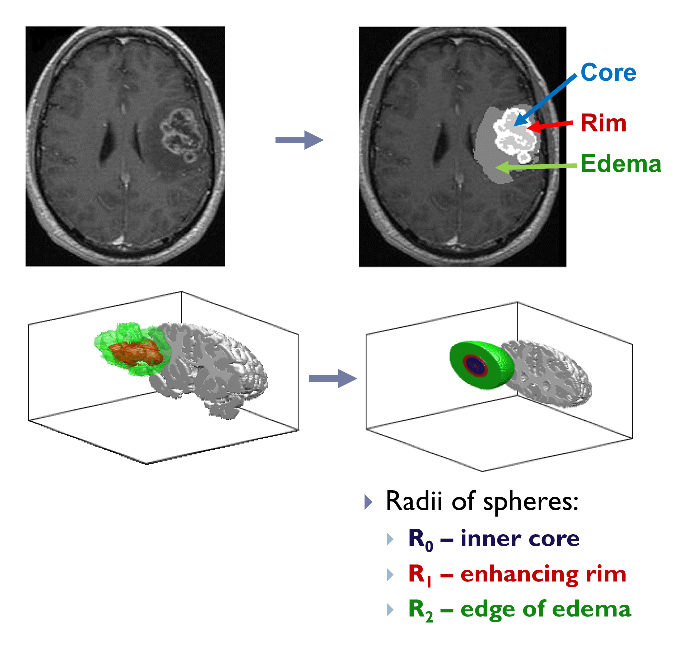
\includegraphics[scale=0.81]{plots/radii_process.eps}
\end{center}
\caption{The top half of the figure shows an example patient MRI registered
to the standard brain domain, with the three tumor segments, necrotic core,
enhancing rim, and tumor-associated edema highlighted on a single 2-D slice.
The full 3-D segmentation, and the equivalent tumor sphere with associated
radii, $R_0$, $R_1$, and~$R_2$, is shown in the lower half.}
\label{fig:radii_process}
\end{figure}

\begin{figure}
\begin{center}
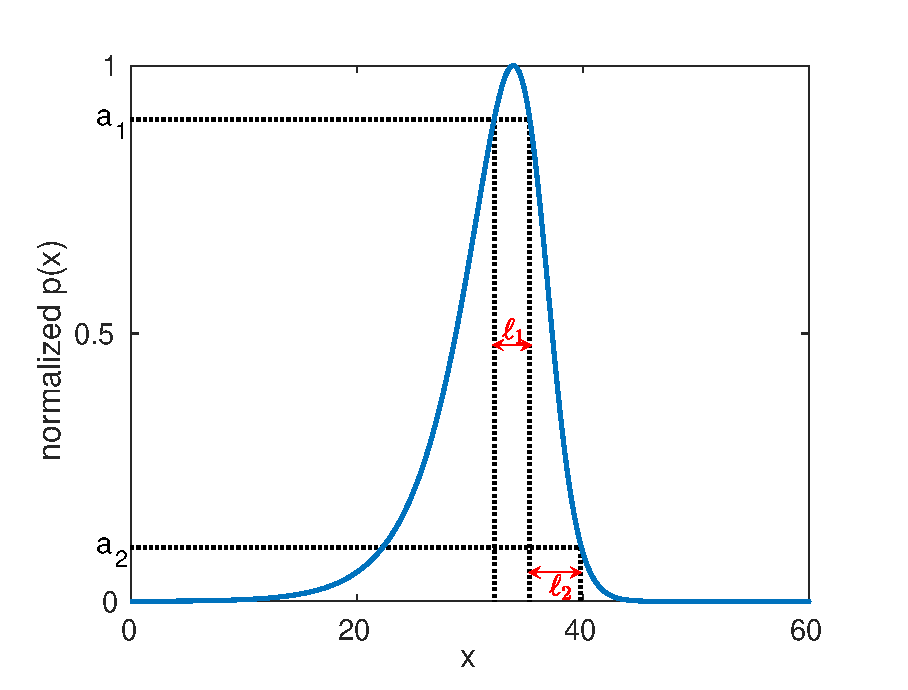
\includegraphics[scale=0.56]{plots/waveprofile.eps}
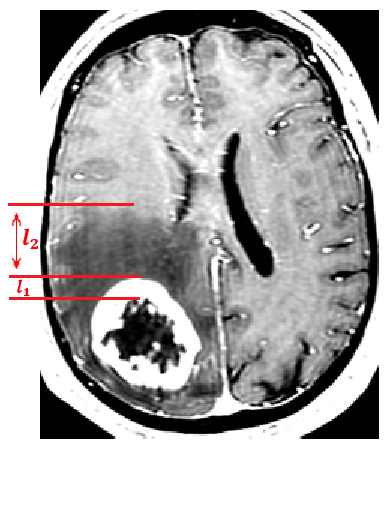
\includegraphics[scale=0.33]{plots/MR.png}
\end{center}
\caption{Left: normalized wave profile generated by the model in the
$z$ coordinate.
Right: tumor profile seen in MR image. Parameter estimation is done by
matching
model-derived quantities, e.g., $\ell_1$ and $\ell_2$, to the corresponding
image-derived ones.}
\label{fig:matchwidth} 
\end{figure}

\section{Results}

Monotonicity is crucial for parameter identifiability, so we
first investigate the monotonicity of $f(\cdot)$ for some specific
choices of $g(w)$ and $\delta(w)$.
Given the restrictions described in Section~\ref{model-sec},
the cumulative density function (CDF) of the Beta distribution family
suits our purposes.  Therefore, we let $g(w)=B(w;\alpha_g,\beta_g)$ and
$\delta(w)=1-B(w;\alpha_{\delta},\beta_{\delta})$, where 
$B(w; \alpha, \beta)$ is the CDF of the beta distribution with shape
parameters $\alpha$ and~$\beta$. By varying $\alpha$ and~$\beta$, we can
get linear, sigmoidal, and concave
up/down curves (see the left pane of Figure~\ref{fig:beta26f}).
Our framework is robust to those choices, that is, the
monotonicity of $f(\hat\rho$), defined by Eq.~(\ref{eq:frhohat}),
is preserved (right pane of Figure~\ref{fig:beta26f}). 
Sigmoidal-shaped growth and death functions ($g$ and~$\delta$, respectively)
may provide biologically realistic response functions to limited growth factors
(most enzymatic reaction rates have sigmoidal
shapes with respect to reactant concentration).  Given this family of
functions, we now consider the question of estimating patient-specific tumor
growth and death rates from MR imaging.

We parameterize our model with patient data in which there is only
one MRI scan before surgery. In Table~\ref{tab:Patient-data-para},
we summarize the image-derived tumor radii and the corresponding parameters
estimated by the method introduced in the previous section.
The parameters $a_1=0.9$ and $a_2=0.1$ are adapted from values found in the
literature~\cite{Swanson2008}, while $p_0=0.02$  and $t^*=60$ days
are hypothetical values.  The parameters vary considerably
among individual patients. 

We compare our approximate quantities to those obtained from the numerical
solution of the model.  As shown in Figure~\ref{fig:comparison-to-numerical},
the approximated results match well with the numerical results except
for some discrepancy for $L_{2}$ when $\hat{\rho}$ is small.  This result
is not a surprise, because the approximation assumes that
$c=2\sqrt{\hat{\rho}}$ is large.  Moreover, the numerical approximation
of $L_{2}$ is prone to errors due to the fixed grid size and large
rate of change around the threshold of~$L_{2}$. Overall, we believe
that our approximation is accurate for the parameter ranges estimated
from the image data.

\begin{figure}
\begin{center}
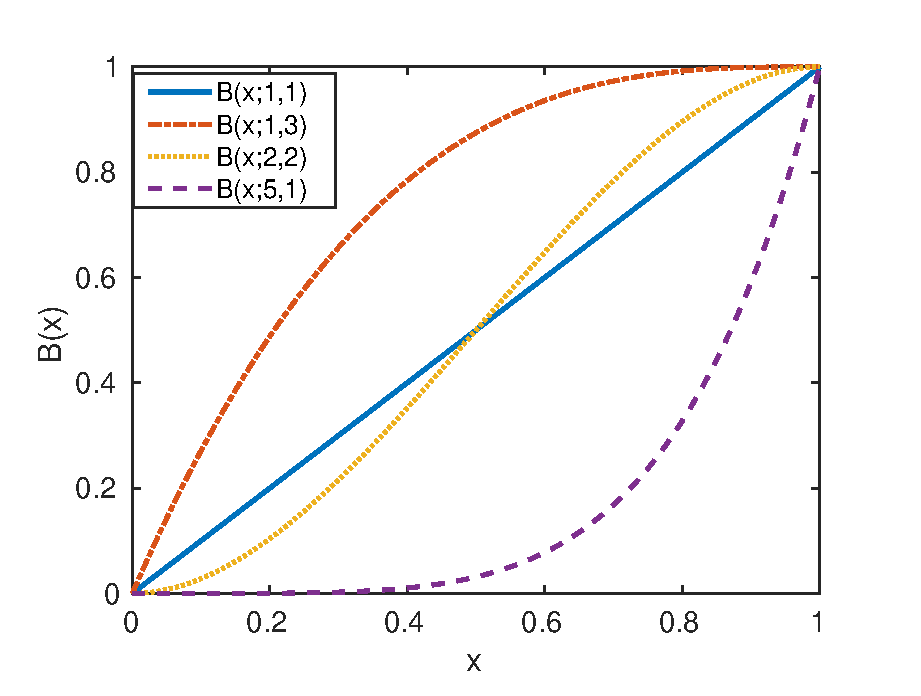
\includegraphics[scale=0.5]{plots/frhok/betas-new}
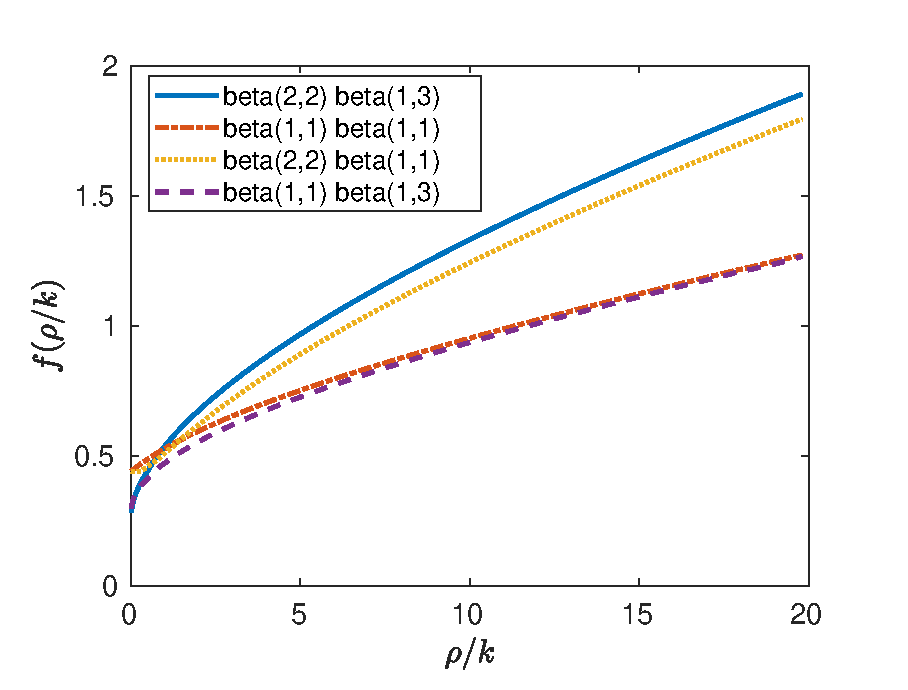
\includegraphics[scale=0.5]{plots/frhok/frhok-new}
\end{center}
\caption{Left: Cumulative distribution functions of some beta distributions. These
functions satisfy Eq.~(\ref{eq:1assume})  and serve as candidates to represent
biological response to limitation of growth factors. Right:
monotonicity of $f(\hat\rho)$ given different choices of $g(w)$ and $\delta(w)$ as
indicated in the legend. All choices lead to a monotonic function $f(\cdot)$ and hence
identifiable parameters.}
\label{fig:beta26f}
\end{figure}

\begin{table}
\begin{center}
\begin{tabular}{ccccccc} \hline
Patient & $R_0$ (mm) & $R_1$ (mm) & $R_2$ (mm) & $D$ ($\mbox{mm}^{2}\mbox{day}^{-1}$)
& $\rho$ ($\mbox{day}^{-1}$) & $k$ ($\mbox{day}^{-1}$) \\ \hline
1 & 14.87 & 20.73 & 27.77 & 0.2852 & 0.2102 & 0.0602 \\
2 & 20.48 & 26.34 & 38.24 & 1.2791 & 0.2624 & 0.3537 \\
3 & 6.61  & 10.91 & 15.24 & 0.0825 & 0.1736 & 0.0327 \\
4 & 22.87 & 26.96 & 37.03 & 0.9825 & 0.2590 & 0.7819 \\
5 & 8.17  & 14.20 & 25.10 & 0.9769 & 0.2520 & 0.2260 \\
6 & 8.29  & 15.83 & 20.35 & 0.0687 & 0.1652 & 0.0106 \\ \hline
\end{tabular}
\end{center}
%(Table body should be created by MS word table function; three-line table is preferred.)
\caption{Radii of equivalent tumor sphere derived from T1 and T2 images and the
corresponding vital parameters estimated by our protocol. We have preset $a_1=0.9$,
$a_2=0.1$, $p_0=0.02$~mm and $t^*=60$ days.}
\label{tab:Patient-data-para} 
\end{table}

\begin{figure}
\begin{center}
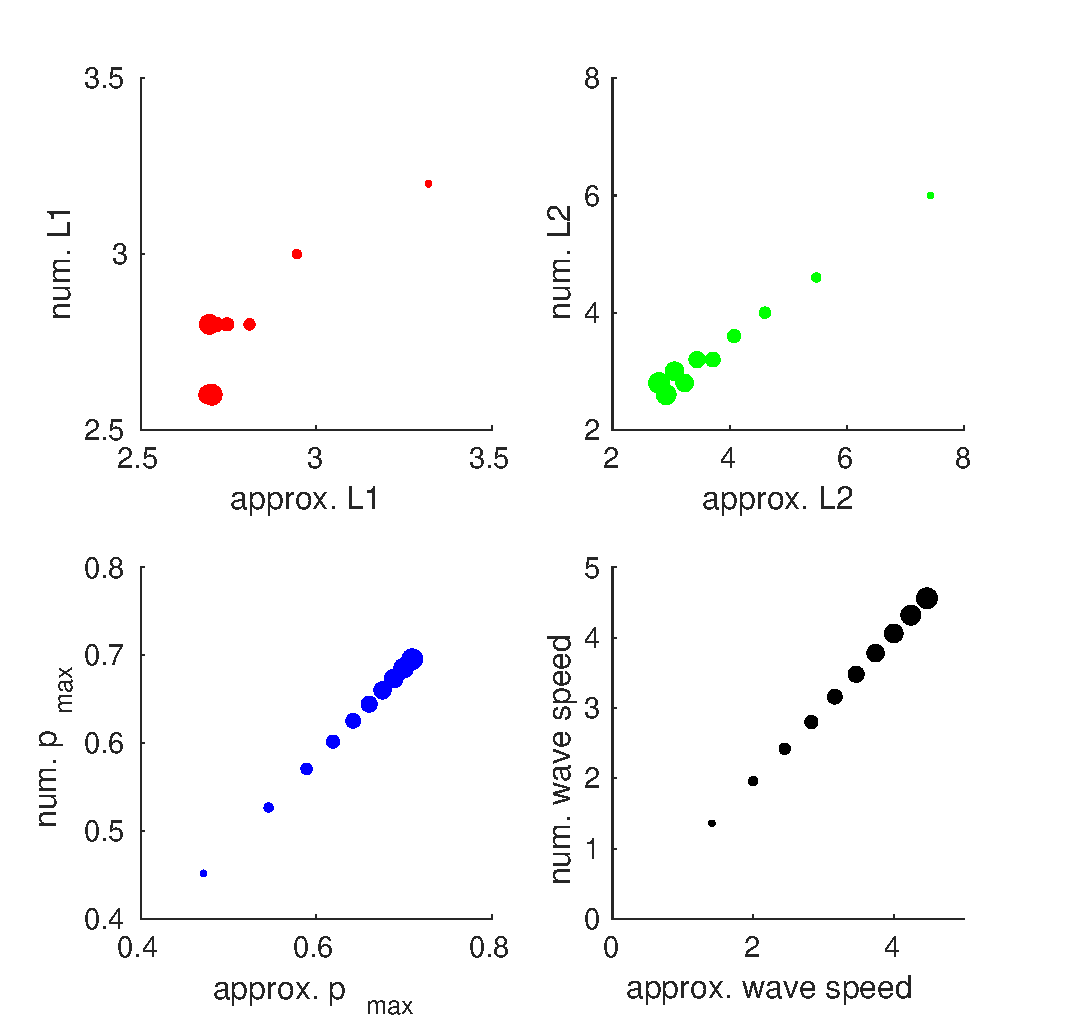
\includegraphics[scale=0.67]{plots/scatterplot-new}
\end{center}
\caption{Scatter plots of approximate wave
profile characteristics (on horizontal axis) verses the ones obtained
by numerical simulation (on vertical axis) for a range of $\hat{\rho}$
from $0.5$ to $5$ by increments of~$0.5$. The size of the dot corresponds
to the value of~$\hat{\rho}$. The dots scatter closely to the diagonal line with
slope~$1$, indicating agreement between the numerical solution and
our approximation.}
\label{fig:comparison-to-numerical}
\end{figure}

\section{Discussion}

In this work, we have extended the Fisher-Kolmogorov reaction-diffusion
model of GBM growth, Eq.~(\ref{fisher-eq}), to explicitly separate the
cancer cell birth and death (or quiescence) processes, which are described
in terms of
generic functions that depend upon an implicit nutrient or growth factor.  We specify
the birth and death processes, $g(w)$ and $\delta(w)$, respectively, by the cumulative
distribution function of a
beta distribution, each uniquely specified by a single parameter, $\rho$ and~$k$. 
Thus, along with the diffusion coefficient, $D$, our model describes cancer
growth via three parameters, $D$, $\rho$, and~$k$, and yields a tumor morphology (in
one dimension) consisting of a necrotic core, a high-density rim, and an outer low
density rim, which we may correlate to three radii, $R_0$, $R_1$, and~$R_2$, that
can be estimated from a single patient MR image.

We have demonstrated that our reaction-diffusion system has a traveling-wave solution,
which is common in such systems.
Studies on this topic date back to the Fisher's work in the 1930s on the spread of
advantageous genes~\cite{Fisher1937}. Rigorous
proof of the existence of traveling wave solution in a reaction-diffusion
system often leads to phase space analysis such as the one on diffusive
Lotka-Volterra equations~\cite{Dunbar1983}.  Although in general a rigorous
proof of a traveling-wave solution is a daunting task, our 
the reduced system is amenable to phase plane analysis, and the orbit that represents
the traveling wave solution can be identified (see appendix).

Via traveling wave analysis, we have developed a method to estimate $D$, $\rho$, and
$k$ from as few as a single magnetic resonance image, based on certain growth
assumptions. We have estimated these parameters for six
patient test cases, as shown in Table~\ref{tab:Patient-data-para}. Because of the
sparsity of imaging data for a typical patient,
parameter identifiability in this case is provided
by the monotonicity of the function  $f(\cdot)$ (as seen in left pane of
Figure~\ref{fig:beta26f});  our approach differs from more common statistical
practices~\cite{Eisenberg2017} that are appropriate when more data are available. 
   
Disaggregating the net cell proliferation into birth and death processes not only
aids in relating (simplified) tumor appearance on MRI to the model parameters, but
it may provide useful valuable information for personalized treatment
design, insofar as chemotherapy and radiotherapy target proliferating cells.
Moreover, the structural information is also potentially useful, as drug dosages
might be selected to ensure penetration through the width
of the proliferating rim. Research along this general line has been conducted using
model (\ref{fisher-eq})~\cite{Kim2017}.

Our analysis uses a more complex description of motility than simple diffusion.
The diffusion term in Eq.~(\ref{eq:main}) belongs to a more general category called
\emph{cross diffusion}~\cite{Madzvamuse2017}.  It represents the phenomenon in which
the gradient in the concentration of one species causes a flux
of another species.  The type of cross diffusion considered in this paper has been
studied in a more general and theoretical context~\cite{Sherratt2000}.  In a
modeling study of avascular tumour growth~\cite{Sherratt2001b}, the authors justified
the adoption of a proportion-based cross diffusion in a tumor-growth model by recognizing
that tumor cell migration is ``contact inhibited'':  the presence
of one type of cell halts the movement of the other. This type of cross diffusion
can cause the solution to become negative~\cite{Madzvamuse2017}, but we have not
encounted this difficulty so far in our numerical simulations.
We conjecture that, for suitable initial conditions,
solutions remain positive, which will be a topic for future study. 
Other types of density-dependent
diffusion have been considered in modeling GBM migration~\cite{Stepien2015}.

Despite the existence of many possible diffusion terms,
the exact form of diffusion does not matter in the one-dimensional analysis, because
the second derivatives are dropped in model~(\ref{eq:1/c^2}).  However,
The diffusion coefficient does play an important role in the linearized
wave head, where it affects the wave speed, and in the characteristic length
where its square root scales the space.  The scale-invariant
part of the wave profile is mostly determined by the exact forms of the
birth and death functions. 

The major contribution of this paper is two novel methods
to make patient-specific estimates of a three-parameter model of
GBM grwoth from the limited MRI data that is typically available in clinical settings.
It is possible to estimate the model parameters from a single pre-surgery image.
Improved estimates may be possible when images are acquired at multiple time points.

As cancers progress, the underlying parameters describing their growth are unlikely to be
static.  Data assimilation refers to basic method of updating parameters as more data is
acquired, and there has been research on applying full-fledged  data assimilation to cancer
modeling~\cite{Kostelich2011,McDaniel2013}.  The methods described in this paper can be
incorporated as part of a future data assimilation system.

\section*{Acknowledgments}
The work is supported
by a grant from Arizona Biomedical Research Commission
and by funds from the Newsome Chair in Neurosurgery Research held by Dr.\ Preul.
The authors would like to thank Dr.\ Leslie Baxter and Dr.\ Leland Hu at the Barrow
Neurological Institute for providing MR images.

%\section*{Conflict of interest}
\bibliography{ref}
\bibliographystyle{AIMS}


%For more questions regarding reference style, please refer to the \href{http://www.ncbi.nlm.nih.gov/books/NBK7256/}{Citing Medicine}.

\section*{Appendix}
\subsection*{Traveling-wave solutions}
In the following, we rigorously establish the existence of traveling-wave solutions in
system~(\ref{eq:pp system}).  We first show that the solutions of
system~(\ref{eq:pp system}) with positive initial values are non-negative and bounded.
 
\noindent
\textbf{Lemma 1.} Assume that $g(w)=wG(w)$, where $G(w)$ is a bounded function. 
Then the solutions of system (\ref{eq:pp system}) with positive initial values are positive and bounded.

\noindent
\emph{Proof:} If $x'=x\,f(t, x)$ and $f$ is a bounded function, then 
$x(t)=x(t_0)\exp \left(\int^t_{t_0} f(s, x(s))\, ds\right)$, which is positive whenever
$x(t_0)>0$. Since
\begin{equation}
\frac{d(p+w)}{dz}=-\delta(w),
\end{equation}
we see that $(p+w)$ is bounded, which implies that both $p$ and $w$ are also bounded.~$\Box$

For any $w^*\in [0,1]$, the point $(0, w^*)$ is an equilibrium of~(\ref{eq:pp system}).

\noindent
\textbf{Theorem 1.}  System~(\ref{eq:pp system}) admits positive traveling-wave solutions
that correspond to heteroclinic orbits connecting the steady state $(0, 1)$ to another
steady state, $(0, w^*)$.

\indent
\emph{Proof:} We have performed a detailed phase plane analysis of~(\ref{eq:pp system})
to show the existence of a trajectory that starts from $(1,0)$ and ends at $(w^{*},0)$,
where $w^*\in [0,1)$.  (See Figure \ref{fig:pp}.)
First we notice that 
\begin{eqnarray}
\frac{dp}{dw} & = & \frac{\delta(w)}{\hat{\rho}g(w)}-1 , \\
\frac{d^2 p}{dw^{2}} & = & \frac{\delta'(w)g(w)-\delta(w)g'(w)}{\hat{\rho} g(w)^{2}},
\end{eqnarray}
Since $g(w)$ and $\delta(w)$ are both positive functions and
$g'(w)>0$ and $\delta'(w)<0$ on $w\in [0,1]$, it follows that
$d^{2}p/dw^{2}<0$ for all $w\in [0,1]$. 

We show first that the trajectory starting from $(1,0)$ will never cross the line $p=1-w$.
Because $g(1)=1$, we have $\delta(1)=0$, and therefore, $dp/dw\big\vert_{w=1}=-1$.
Since $d^2 p/dw^{2}<0$, the slope of a trajectory with $w<1$ will be greater than
$-1$, which means it will not cross the line $p=1-w$.
Also, because the solution components stay positive, the trajectory starting
from $(1,0)$ will never cross the $p$-axis from right to left. 

Because the functions $g$ and $\delta$ are monotone, 
there is a unique value $w^{\dagger}\in (0, 1)$ such that 
$dp/dw\big\vert_{w=w^{\dagger}}=0$. 
Moreover, $dp/dw\big\vert_{1>w>w^{\dagger}}>0$ while
$dp/dw\big\vert_{0<w<w^{\dagger}}<0$.

Insofar as $w$ is strictly decreasing and bounded from below by 0, 
there exists some $w^*\in(0,1)$ such that $\lim_{z \rightarrow \infty} w(z)=w^*$. 
We claim that $w^*<w^{\dagger}$.
Otherwise, $p$ is a non-decreasing function, which implies that the trajectory approaches a positive steady state $E^*=(p^*, w^*)$.   
However, the system~(\ref{eq:pp system}) does not admit any positive steady states. 

Let $a \in (w^*, w^{\dagger})$ and $b=\hat{\rho}g(a)-\delta(a) <0$.   Since
$\lim_{z \rightarrow \infty}w(z)=w^*$, there is a $z^*>0$ such that for
$z \geq z^*$ and $w<a$.  Therefore, for $z \geq z^*$, 
$dp/dz <bp$, which implies that $\lim_{z \rightarrow \infty} p(z)=0$.
Hence, system~(\ref{eq:pp system}) admits positive traveling-wave solutions that
correspond to heteroclinic orbits connecting the steady state $(0, 1)$ to 
another steady state, $(0, w^*)$.~$\Box$

\subsection*{Rim width}
The trajectory in Figure~\ref{fig:pp} corresponds to a traveling wave profile in the
$z$~coordinate as shown on the left pane of Figure~\ref{fig:matchwidth}. Because of our
choice of nondimensionlization, $x=-\left(2 \sqrt{D\rho}\,/k\right) z$, 
by definition we have the rim width in the dimensional form  
\begin{eqnarray}
\ell_1= \frac{2 \sqrt{D\rho}}{k} (z_1^+ - z_1^-) = \frac{2 \sqrt{D\rho}}{k} \int_{z_1^-}^{z_1^+} dz\
\end{eqnarray}
where $p(z^{\pm}_1)=a_1 p_{\max}$.  We have taken $p$ as a function of~$z$
(cf.\ the left pane of Figure~\ref{fig:matchwidth}). We can also take $w$ as a function of
$z$ to make a change of variable to the above integral, which gives Eq.~(\ref{eq:l1}).
A similar argument applies to (\ref{eq:l2}).
 
\subsection*{Derivation of $R_1^*$ and $R_2^*$}

\begin{figure}
\begin{center}
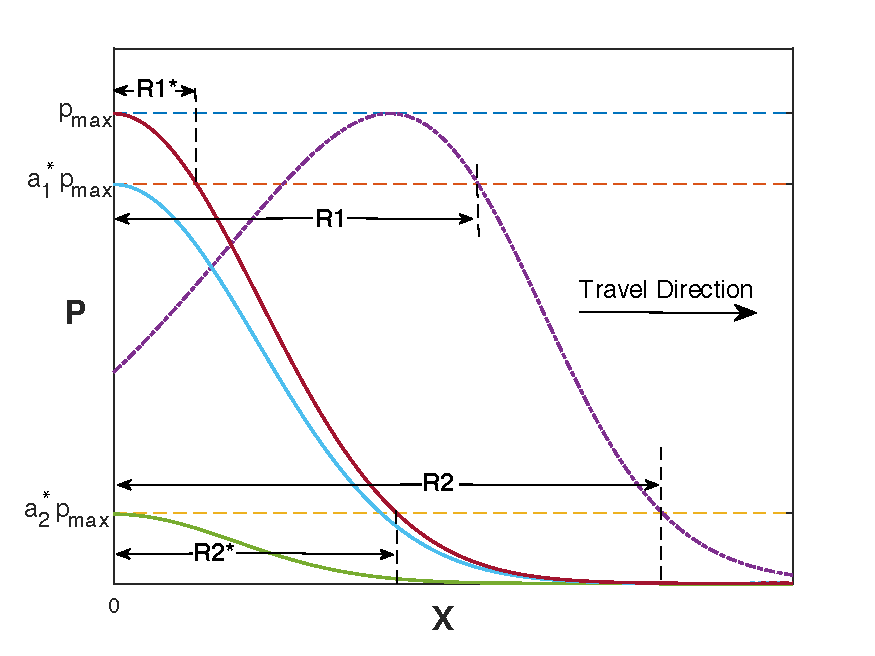
\includegraphics[scale=0.90]{plots/wave-edited.pdf}
\end{center}
\caption{The transition of wave profile based on the two-stage tumor growth model. The
dotted (purple) curve represents a stable wave profile generated by
system~(\ref{eq:pp system}). The solid curves are generated by Eq.~(\ref{eq:exp system})
and represent the tumor's exponential growth phase.
The stable wave profile is formed after the exponential growth curve reaches
$p_{\mbox{\scriptsize max}}$ (red solid curve).}
\label{fig:wave}
\end{figure}

Tumor growth can be separated into two stages. First, the tumor cells grow exponentially
until the cell density is high enough ($p_{\mbox{\scriptsize max}}$) to form 
a stable wave profile. Afterward, the growth of tumor cells is described
by~(\ref{eq:pp system}).
The radii $R_1$ and $R_2$ are observed from clinical MRI data and correspond respectively
to the
distance from the center of the tumor to the edge of the enhancing rim and to the edge
of the edematous region on T2 imaging; they correspond to tumor dynamics
before the stable wave profile has formed (cf.\ Figure~\ref{fig:wave}). 

During the exponential growth phase, say from $0<t<t^*$, quiescence is negligible and the governing equation of tumor cell density is 
\begin{eqnarray}\label{eq:exp system}
\pardiff{p}{t} =  D\frac{1}{r^2} \pardiff{}{r} \left(r^2 \pardiff{p}{r}\right) + \rho p,
\end{eqnarray}
where spherical symmetry is used, as we assume that the tumor is spherical when
its radius is small.
This linear equation has the Green's function 
\begin{eqnarray}
p(r,t)=\frac{1}{(4 \pi D t)^{3/2}}\, \exp\left(\rho t - \frac{r^2}{4Dt}\right) 
\end{eqnarray}
(see, e.g., \cite{KotBook} Page 314 and \cite{BrittonBook} Page 285).
Suppose that the tumor starts at $t=0$ as a point source with density~$p_0$.
It follows that at $t=t^*$, the position of the tumor front at density $p=a_i$  is 
given by Eq.~(\ref{eq:Rstar}). 

\end{document}

%\bibliographystyle{AIMS}
%\bibliography{ref}
\providecommand{\href}[2]{#2}
\providecommand{\arxiv}[1]{\href{http://arxiv.org/abs/#1}{arXiv:#1}}
\providecommand{\url}[1]{\texttt{#1}}
\providecommand{\urlprefix}{URL }
\begin{thebibliography}{10}

\bibitem{BrittonBook}
\newblock N.~F. Britton,
\newblock \emph{{Essential mathematical biology}},
\newblock Springer, 2003.

\bibitem{Canosa1973}
\newblock J.~Canosa,
\newblock {On a Nonlinear Diffusion Equation Describing Population Growth},
\newblock \emph{IBM Journal of Research and Development}, \textbf{17} (1973),
  307--313,
\newblock \urlprefix\url{http://ieeexplore.ieee.org/document/5391351/}.

\bibitem{Dunbar1983}
\newblock S.~Dunbar,
\newblock {Travelling wave solutions of diffusive Lotka-Volterra equations},
\newblock \emph{Journal of Mathematical Biology}, \textbf{17} (1983), 11--32,
\newblock \urlprefix\url{http://link.springer.com/10.1007/BF00276112}.

\bibitem{Eikenberry2009}
\newblock S.~E. Eikenberry, T.~Sankar, M.~C. Preul, E.~J. Kostelich, C.~J.
  Thalhauser and Y.~Kuang,
\newblock {Virtual glioblastoma: Growth, migration and treatment in a
  three-dimensional mathematical model},
\newblock \emph{Cell Proliferation}, \textbf{42} (2009), 511--528.

\bibitem{Eisenberg2017}
\newblock M.~C. Eisenberg and H.~V. Jain,
\newblock {A confidence building exercise in data and identifiability: Modeling
  cancer chemotherapy as a case study},
\newblock \emph{Journal of Theoretical Biology}, \textbf{431} (2017), 63--78,
\newblock
  \urlprefix\url{https://www.sciencedirect.com/science/article/pii/S0022519317303454?via{\%}3Dihub}.

\bibitem{Fedorov2012}
\newblock A.~Fedorov, R.~Beichel, J.~Kalpathy-Cramer, J.~Finet, J.-C.
  Fillion-Robin, S.~Pujol, C.~Bauer, D.~Jennings, F.~Fennessy, M.~Sonka,
  J.~Buatti, S.~Aylward, J.~V. Miller, S.~Pieper and R.~Kikinis,
\newblock {3D Slicer as an image computing platform for the Quantitative
  Imaging Network},
\newblock \emph{Magnetic Resonance Imaging}, \textbf{30} (2012), 1323--1341,
\newblock
  \urlprefix\url{https://www.sciencedirect.com/science/article/pii/S0730725X12001816?via{\%}3Dihub}.

\bibitem{FISHER1937}
\newblock R.~A. Fisher,
\newblock {The wave of advance of advantageous genes},
\newblock \emph{Annals of Eugenics}, \textbf{7} (1937), 355--369,
\newblock
  \urlprefix\url{http://doi.wiley.com/10.1111/j.1469-1809.1937.tb02153.x}.

\bibitem{Gerlee2016}
\newblock P.~Gerlee and S.~Nelander,
\newblock {Travelling wave analysis of a mathematical model of glioblastoma
  growth},
\newblock \emph{Mathematical Biosciences}, \textbf{276} (2016), 75--81,
\newblock
  \urlprefix\url{https://www.sciencedirect.com/science/article/abs/pii/S0025556416000602?via{\%}3Dihub}.

\bibitem{Gilbert2013}
\newblock M.~R. Gilbert, M.~Wang, K.~D. Aldape, R.~Stupp, M.~E. Hegi, K.~A.
  Jaeckle, T.~S. Armstrong, J.~S. Wefel, M.~Won, D.~T. Blumenthal, A.~Mahajan,
  C.~J. Schultz, S.~Erridge, B.~Baumert, K.~I. Hopkins, T.~Tzuk-Shina, P.~D.
  Brown, A.~Chakravarti, W.~J. Curran and M.~P. Mehta,
\newblock {Dose-dense temozolomide for newly diagnosed glioblastoma: a
  randomized phase III clinical trial.},
\newblock \emph{Journal of clinical oncology : official journal of the American
  Society of Clinical Oncology}, \textbf{31} (2013), 4085--91,
\newblock \urlprefix\url{http://ascopubs.org/doi/10.1200/JCO.2013.49.6968
  http://www.ncbi.nlm.nih.gov/pubmed/24101040
  http://www.pubmedcentral.nih.gov/articlerender.fcgi?artid=PMC3816958}.

\bibitem{Harley2014}
\newblock K.~Harley, P.~van Heijster, R.~Marangell, G.~J. Pettet and
  M.~Wechselberger,
\newblock {Existence of Traveling Wave Solutions for a Model of Tumor
  Invasion},
\newblock \emph{SIAM Journal on Applied Dynamical Systems}, \textbf{13} (2014),
  366--396,
\newblock \urlprefix\url{http://epubs.siam.org/doi/10.1137/130923129}.

\bibitem{Jackson2015a}
\newblock P.~R. Jackson, J.~Juliano, A.~Hawkins-Daarud, R.~C. Rockne and K.~R.
  Swanson,
\newblock {Patient-Specific Mathematical Neuro-Oncology: Using a Simple
  Proliferation and Invasion Tumor Model to Inform Clinical Practice},
\newblock \emph{Bulletin of Mathematical Biology}, \textbf{77} (2015),
  846--856,
\newblock \urlprefix\url{http://link.springer.com/10.1007/s11538-015-0067-7}.

\bibitem{Kim2017}
\newblock M.~Kim, J.~Kotas, J.~Rockhill, M.~Phillips, M.~Kim, J.~Kotas,
  J.~Rockhill and M.~Phillips,
\newblock {A Feasibility Study of Personalized Prescription Schemes for
  Glioblastoma Patients Using a Proliferation and Invasion Glioma Model},
\newblock \emph{Cancers}, \textbf{9} (2017), 51,
\newblock \urlprefix\url{http://www.mdpi.com/2072-6694/9/5/51}.

\bibitem{Kostelich2011}
\newblock E.~J. Kostelich, Y.~Kuang, J.~M. McDaniel, N.~Z. Moore, N.~L.
  Martirosyan and M.~C. Preul,
\newblock {Accurate state estimation from uncertain data and models: an
  application of data assimilation to mathematical models of human brain
  tumors},
\newblock \emph{Biology Direct}, \textbf{6} (2011), 64,
\newblock
  \urlprefix\url{http://biologydirect.biomedcentral.com/articles/10.1186/1745-6150-6-64}.

\bibitem{KotBook}
\newblock M.~Kot,
\newblock \emph{{Elements of mathematical ecology}},
\newblock Cambridge University Press, 2001,
\newblock
  \urlprefix\url{https://www.cambridge.org/us/academic/subjects/life-sciences/ecology-and-conservation/elements-mathematical-ecology?format=PB{\&}isbn=9780521001502}.

\bibitem{Kuang}
\newblock Y.~Kuang, J.~D. Nagy and S.~E. Eikenberry,
\newblock \emph{{Introduction to mathematical oncology}},
\newblock Chapman and Hall/CRC.

\bibitem{Madzvamuse2017}
\newblock A.~Madzvamuse, R.~Barreira and A.~Gerisch,
\newblock {Cross-Diffusion in Reaction-Diffusion Models: Analysis, Numerics,
  and Applications},
\newblock Springer, Cham, 2017,
\newblock 385--392,
\newblock
  \urlprefix\url{http://link.springer.com/10.1007/978-3-319-63082-3{\_}61}.

\bibitem{Martirosyan2015}
\newblock N.~L. Martirosyan, E.~M. Rutter, W.~L. Ramey, E.~J. Kostelich,
  Y.~Kuang and M.~C. Preul,
\newblock {Mathematically modeling the biological properties of gliomas: A
  review},
\newblock \emph{Mathematical Biosciences and Engineering}, \textbf{12} (2015),
  879--905,
\newblock
  \urlprefix\url{http://aimsciences.org/journals/displayArticlesnew.jsp?paperID=11020}.

\bibitem{McDaniel2013}
\newblock J.~McDaniel, E.~Kostelich, Y.~Kuang, J.~Nagy, M.~C. Preul, N.~Z.
  Moore and N.~L. Matirosyan,
\newblock {Data Assimilation in Brain Tumor Models},
\newblock Springer, New York, NY, 2013,
\newblock 233--262,
\newblock
  \urlprefix\url{http://link.springer.com/10.1007/978-1-4614-4178-6{\_}9}.

\bibitem{Neal2013}
\newblock M.~L. Neal, A.~D. Trister, T.~Cloke, R.~Sodt, S.~Ahn, A.~L. Baldock,
  C.~A. Bridge, A.~Lai, T.~F. Cloughesy, M.~M. Mrugala, J.~K. Rockhill, R.~C.
  Rockne and K.~R. Swanson,
\newblock {Discriminating Survival Outcomes in Patients with Glioblastoma Using
  a Simulation-Based, Patient-Specific Response Metric},
\newblock \emph{PLoS ONE}, \textbf{8} (2013), e51951,
\newblock \urlprefix\url{https://dx.plos.org/10.1371/journal.pone.0051951}.

\bibitem{Norden2006}
\newblock A.~D. Norden and P.~Y. Wen,
\newblock {Glioma therapy in adults},
\newblock \emph{The neurologist}, \textbf{12} (2006), 279--92,
\newblock \urlprefix\url{http://www.ncbi.nlm.nih.gov/pubmed/17122724}.

\bibitem{Penny2007}
\newblock W.~D. Penny, K.~J. K.~J. Friston, J.~Ashburner, S.~Kiebel and
  T.~Nichols,
\newblock \emph{{Statistical parametric mapping : the analysis of funtional
  brain images}},
\newblock Elsevier/Academic Press, 2007.

\bibitem{Sherratt2000}
\newblock J.~A. Sherratt,
\newblock {Wavefront propagation in a competition equation with a new motility
  term modelling contact inhibition between cell populations},
\newblock \emph{Proceedings of the Royal Society of London. Series A:
  Mathematical, Physical and Engineering Sciences}, \textbf{456} (2000),
  2365--2386,
\newblock
  \urlprefix\url{http://www.royalsocietypublishing.org/doi/10.1098/rspa.2000.0616}.

\bibitem{Sherratt2001b}
\newblock J.~A. Sherratt and M.~A. Chaplain,
\newblock {A new mathematical model for avascular tumour growth},
\newblock \emph{Journal of Mathematical Biology}, \textbf{43} (2001), 291--312,
\newblock \urlprefix\url{http://link.springer.com/10.1007/s002850100088}.

\bibitem{Stepien2015}
\newblock T.~L. Stepien, E.~M. Rutter and Y.~Kuang,
\newblock {A data-motivated density-dependent diffusion model of in vitro
  glioblastoma growth.},
\newblock \emph{Mathematical biosciences and engineering : MBE}, \textbf{12}
  (2015), 1157--72,
\newblock \urlprefix\url{http://www.ncbi.nlm.nih.gov/pubmed/26775861}.

\bibitem{Stepien2018}
\newblock T.~L. Stepien, E.~M. Rutter and Y.~Kuang,
\newblock {Traveling Waves of a Go-or-Grow Model of Glioma Growth},
\newblock \emph{SIAM Journal on Applied Mathematics}, \textbf{78} (2018),
  1778--1801,
\newblock \urlprefix\url{https://epubs.siam.org/doi/10.1137/17M1146257}.

\bibitem{Stupp2005}
\newblock R.~Stupp, W.~P. Mason, M.~J. van~den Bent, M.~Weller, B.~Fisher,
  M.~J. Taphoorn, K.~Belanger, A.~A. Brandes, C.~Marosi, U.~Bogdahn,
  J.~Curschmann, R.~C. Janzer, S.~K. Ludwin, T.~Gorlia, A.~Allgeier,
  D.~Lacombe, J.~G. Cairncross, E.~Eisenhauer and R.~O. Mirimanoff,
\newblock {Radiotherapy plus Concomitant and Adjuvant Temozolomide for
  Glioblastoma},
\newblock \emph{New England Journal of Medicine}, \textbf{352} (2005),
  987--996,
\newblock \urlprefix\url{http://www.nejm.org/doi/abs/10.1056/NEJMoa043330}.

\bibitem{Swanson2011}
\newblock K.~R. Swanson, R.~C. Rockne, J.~Claridge, M.~A. Chaplain, E.~C.
  Alvord and A.~R.~A. Anderson,
\newblock {Quantifying the Role of Angiogenesis in Malignant Progression of
  Gliomas: In Silico Modeling Integrates Imaging and Histology},
\newblock \emph{Cancer Research}, \textbf{71} (2011), 7366--7375,
\newblock \urlprefix\url{http://www.ncbi.nlm.nih.gov/pubmed/21900399
  http://www.pubmedcentral.nih.gov/articlerender.fcgi?artid=PMC3398690
  http://cancerres.aacrjournals.org/cgi/doi/10.1158/0008-5472.CAN-11-1399}.

\bibitem{Swanson2008}
\newblock K.~R. Swanson, R.~C. Rostomily and E.~C. Alvord,
\newblock {A mathematical modelling tool for predicting survival of individual
  patients following resection of glioblastoma: a proof of principle},
\newblock \emph{British Journal of Cancer}, \textbf{98} (2008), 113--119,
\newblock \urlprefix\url{http://www.nature.com/articles/6604125}.

\end{thebibliography}


\end{document}
